\chapter{Support Vector Machines}

\section{Introduction}
Support Vector Machines, SVM, is another successful algorithm that has proven and demonstrated excellent results in many different real-world applications. Its foundations date back to relatively early times, beginning in 1963, when the Russian (Soviet) mathematician Vladimir Vapnik (along with Alexey Chervonenkis, Alexander Lerner, and others) published works on statistical learning and pattern recognition.

These works gradually gave rise to one of the current successful algorithms based on the theory of linear algebra [31]. In principle, SVM is a classification algorithm aimed at separating two classes using a hyperplane - a linear classifier. There are several ways to place a hyperplane (or a straight line in twodimensional space) that separates elements of two classes. The problem is that if such an option exists, one can generally create infinitely many such boundaries for a given set of training examples; see Figure 10.1.

The figure shows here only three of the infinitely many possible separating linear boundaries, $a, b$, and $c$, found by some method. For the training data (which does not include that misclassified item), all three boundaries are perfect, so any of them can be selected. However, if a new element belonging to the white ring class appears, two of the initially set boundaries ( $a$ and $b$ ) put it wrongly in the black rings. So, is the boundary marked $c$ optimal? Or not? The question is whether an optimal solution can be found based on training examples to minimize such potential future misclassifications as much as possible - hence the optimum hyperplane is such that the minimum value of the distance of the points from that plane is as large as possible.

\begin{figure}[!ht]
\begin{center}
  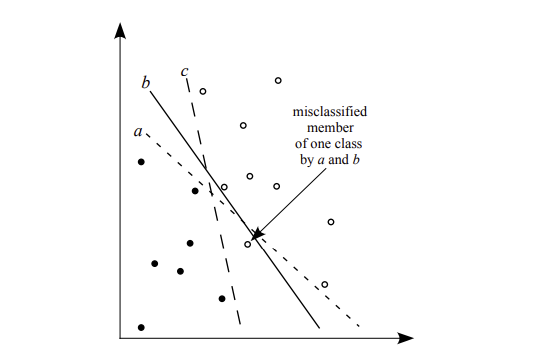
\includegraphics[width=0.8\textwidth]{chapter/chapter10/figure10_1.png}
\caption{Some of possible linear boundaries can wrongly separate a class member.}
\label{fig10.1}
\end{center}
\end{figure}

\begin{figure}[!ht]
\begin{center}
  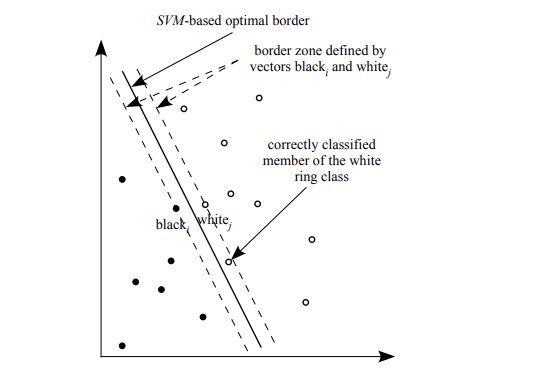
\includegraphics[width=0.8\textwidth]{chapter/chapter10/figure10_2.png}
\caption{The optimal border found by SVM passes through the center of the border zone defined by the $black_i$ and $white_j$ support vectors.}
\label{fig10.2}
\end{center}
\end{figure}

Support Vector Machines algorithm can be offered as the right answer - see the illustration Figure 10.2, which uses the same black and white samples as Figure 10.1.

First, according to the SVM's idea, it is necessary to find the widest zone (belt) separating both classes. Suitably selected examples called support vectors determine the edges of this zone.

Next the optimum boundary (hyper)plane can be placed through the center of the zone. Of course, without knowing all the possible cases (which can theoretically be infinite), this may not guarantee absolute faultlessness for the future classifications of the cases that are not available for the training process, but it increases the chance that even very near-border cases will be classified correctly.

\section{Support Vector Machines Principles}
The linear function behaviour, unlike the nonlinear one, has its shape firmly predetermined. This simplifies the whole situation in the application of linear separation because the nonlinear pattern can be arbitrary and its correct selection for a boundary may not often be quite obvious. Therefore, if possible (and also in accordance with Occam's razor), it is appropriate to use the linear function.

The principles of the Support Vector Machines algorithm are based on a relatively large non-trivial mathematical apparatus combining a number of sectors (especially linear algebra, kernel functions, nonlinear optimization). Unfortunately, due to limitations of space, it is not possible to reproduce details here. The reader may try the example presented below to apply SVM to the sample data, play with parameters (for example, the type of kernel function - linear, polynomial, radial) and, in the case of deeper interest in the basics, get familiar with the details in the literature - some links to excellent resources are presented in References.

\subsection{Finding Optimal Separation Hyperplane}
The first problem, as indicated with the help of Figure 10.1 and Figure 10.2, is the problem of locating the separating hyperplane as best as possible by finding the boundary zone - that is, finding, among all the samples, those whose combinations would create the widest zone. Obviously, this is computationally very demanding and it is not possible to do it in practice by trying all possible combinations because of computational complexity - for some applications, there might be millions of training samples, or more.

Thus, certain simplifying techniques and heuristics must be used to overcome this high complexity. Various implementations of SVM use the optimization method known as quadratic programming (optimizing a quadratic function of variables with linear constraints); for an example, see [\cite{ref24}], which is a special case of nonlinear programming.

\subsection{Nonlinear Classification and Kernel Functions}
The second problem is that linear boundaries are often not sufficient because the task inherently requires a nonlinear boundary - and this leads to difficulty in determining a shape of the nonlinear boundary, being possibly stuck in local extremes as it is known for some alternative algorithms (typically, artificial neural networks with neurons having a nonlinear transfer function). A surprising solution may seem to be that when a curve cannot be straightened in a given space to provide a linear separation, it is possible to adjust, "incurvate," the task space somehow in order to use a hyperplane.

This problem relating to nonlinear classification is solved by so called kernel transformation based on kernel functions [\cite{ref30}, \cite{ref243}], which is the SVM's key to adapting the properties of the space under investigation: the transformation of the original space of the data attributes into the space of transformed attributes - typically, the space of higher dimension. This kernel transformation makes it possible to convert the initially linearly non-separable task into a linearly separable one, to which an optimization algorithm can be applied in order to find the separating hyperplane.

The transformation process is illustrated in Figure 10.3 (from onedimensional to two-dimensional space) and Figure 10.4 (from two-dimensional to three-dimensional space).

In one-dimensional space, there is evidently no possibility of separating black and white circle classes from one another using a hyperplane (here, a point somewhere on the $x_{1}$ axis). Only after the transformation into a twodimensional space, where a new artificial coordinate $x_{2}$ is created as a function of $x_{1}, x_{2}=f\left(x_{1}\right)$, and the points are distributed on a parabola (kernel function), can the necessary boundary zone be found and in the middle of it, a separating boundary (the grey belt) of both classes.

Similarly, it is for the transformation from two-dimensional space (one class is bounded by an oval) into three-dimensional space with a new artificial dimension $x_{3}=f\left(x_{1}, x_{2}\right)$, where the white and black circles are placed on the surface of the paraboloid (kernel function).

The transformation of vectors (training samples) from the Euclidean space, where it is not possible to separate both classes linearly, into another Euclidean space, where it is already possible, is done by kernel functions. The essence is that it is not necessary to know the representation of the $\Phi$ transformation function, but it is sufficient to calculate only the scalar product of the $\Phi$ function applied to the transformed vectors, using the kernel function $K$ :

$$
K\left(\vec{x}_{i}, \vec{x}_{j}\right)=\Phi\left(\vec{x}_{i}\right) \cdot \Phi\left(\vec{x}_{j}\right) .
$$

For example, for the linear transformation, $K\left(\vec{x}_{i}, \vec{x}_{j}\right)=\vec{x}_{i} \cdot \vec{x}_{j}$, for the polynomial function of degree $d$ it is $K\left(\vec{x}_{i}, \vec{x}_{j}\right)=\left(\vec{x}_{i} \cdot \vec{x}_{j}+1\right)^{d}$, and so like.

\begin{figure}[H]
\begin{center}
  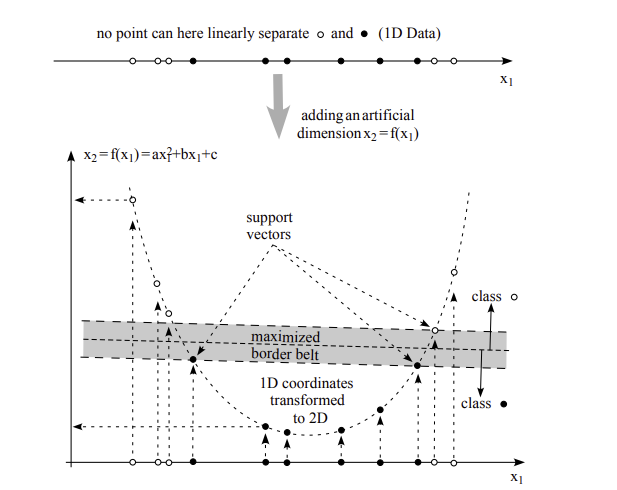
\includegraphics[width=0.8\textwidth]{chapter/chapter10/figure10_3.png}
\captionsetup{labelformat=empty}
\caption{\textbf{Figure 10.3:} The Support Vector Machine (SVM) principle of creating the linear boundary between classes using the specific SVM transformation into a space with a larger number of dimensions. The above example illustrates transformation from 1D to 2D space.}
\label{fig10.3}
\end{center}
\end{figure}

Indeed, the use of a scalar product greatly simplifies and accelerates the computational process. A reader can find additional information in [59, 111].

\subsection{Multiclass SVM Classification}
The third problem might be that SVM procedure can separate only two classes (one above, the other, below a hyperplane) from each other. However, in reality, there may possibly be more than two classes.

At first glance, there are two simple straightforward methods based on the transformation to the binary case: one-against-one (all individual couples are trained against each other) and one-against-all (a particular class is trained against the rest of classes).

The former method suffers mainly from high computational complexity as well as from scale variability of the confidence values that may differ between the binary classifiers, while the latter method typically suffers from the unbalanced number of training samples even if the individual training sets are balanced.

\begin{figure}[H]
\begin{center}
  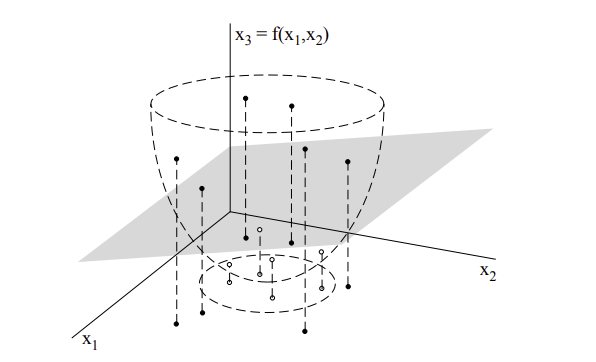
\includegraphics[width=0.8\textwidth]{chapter/chapter10/figure10_4.png}
\captionsetup{labelformat=empty}
\caption{\textbf{Figure 10.4:} Creating a hyperplane (marked here in gray) that separates two classes using the transformation from the original 2D to artificial 3D space.}
\label{fig10.4}
\end{center}
\end{figure}

Apart from the two above-mentioned methods, extensions to handle the multiclass classification case have been proposed. In these extensions, additional parameters and constraints are added to the optimization problem to handle the separation of the different classes. Details and additional references may be found in literature, for example [\cite{ref274}].

\subsection{SVM Summary}
Modern SVM-based classification systems can solve all the mentioned issues. Even if SVM is generally computationally demanding, its result is usually worthwhile.

One of SVM's big advantages (unlike, for example, the $k$-NN algorithm mentioned earlier) is that after training, only the found support vectors need to be stored for future classifications, which in most applications is typically just a fraction of all provided training samples. The real-time classification then proceeds very fast.

Because of the linearity, training always finds a global (optimal) solution with reproducible results, independent of the choice of a starting point (unlike, for example, artificial neural networks).

On the other hand, there are also some problems and limitations. The correct function of the SVM depends largely on the appropriate choice of kernel function, which is not always easy to find. For very large numbers of support vectors, there\\
is a problem with speed and memory requirements. Appropriate algorithms for their solution, namely because of the current group of problems connected with Big Data, are still under investigation.

\subsection{SVM in R}
Using the same set of training samples, the classification with one of the available implementations of SVM in the R-system is demonstrated here. There are several packages/libraries available. An implementation from the package e1071 was selected for the demonstration of the SVN functionality because it provided the best classification results for the demonstration data. The applied script follows below. After the preparation of training and test data, the model based on training samples is created using the function svm\_model(). The linear kernel function selected here; however, an interested reader may try alternative kernel functions (radial basis function RBF, sigmoidal, or polynomial). The parameter type="C-classification" is used for binary classifications, which is also the presented example. The complete parameter description of e1071 is available in [\cite{ref193}].

The advanced implementation provides rich capabilities, but it takes some time to study and test combinations of different parameters depending on the data being analyzed - for reasons of space, it is not possible to provide detailed instructions here, but the Internet can help find the necessary information.

\begin{verbatim}
library(e1071)
# loading the data
data <- read.csv("BookReviews.csv", header=TRUE)
# converting the data to a matrix
dtm <- as.matrix(data)
# removing the object data (unnecessary from now)
rm(data)
# number of instances
n <- dim(dtm)[1]
# number of attributes
m <- dim(dtm)[2]
# indexes of 100 testing samples
\end{verbatim}

\begin{verbatim}
number_of_test_samples <- 100
test_index <- 1:number_of_test_samples
# selecting training samples
train_data <- dtm[-test_index, 1:(m-1)]
train_labels <- dtm[-test_index, m]
# selecting testing samples
test_data <- dtm[test_index, 1:(m-1)]
test_labels <- dtm[test_index, m]
# training a SVM model for classification
svm_model <- svm(train_data,
    train_labels,
    type="C-classification",
    kernel="linear")
# calculating class predictions
predictions<-predict(svm_model, test_data, type="class")
# creating a confusion matrix
cm <- table(test_labels, predictions)
print("Confusion matrix")
print(cm)
# number of instances
n <- sum(cm)
# number of correctly classified instances for each class
correct <- diag(cm)
# numbers of instances in each class
instances_in_classes <- apply(cm, 1, sum)
# numbers of each class predictions
class_predictions <- apply(cm, 2, sum)
# accuracy
accuracy <- sum(correct)/n
# precision per class
precision <- correct/class_predictions
\end{verbatim}

\begin{verbatim}
# recall per class
recall <- correct/instances_in_classes
# F1-measure per class
f1 <- 2 * precision * recall / (precision + recall)
# printing summary information for all classes
df <- data.frame(precision, recall, f1)
print("Detailed classification metrics")
print(df)
print(paste("Accuracy:", accuracy))
# macroaveraging
print("Macro-averaged metrics")
print(colMeans(df))
# microaveraging
print("Micro-averaged metrics")
print(apply(df, 2, function (x)
            weighted.mean(x, w=instances_in_classes)))
\end{verbatim}

Output:\\[0pt]
[1] "Confusion matrix" predictions

\begin{center}
\begin{tabular}{rrr}
test\_labels & 0 & 1 \\
0 & 40 & 17 \\
1 & 12 & 31 \\
\end{tabular}
\end{center}

[1] "Detailed classification metrics"

\begin{center}
\begin{tabular}{rrrr}
 & precision & recall & f1 \\
0 & 0.7692308 & 0.7017544 & 0.7339450 \\
1 & 0.6458333 & 0.7209302 & 0.6813187 \\
\end{tabular}
\end{center}

[1] "Accuracy: 0.71"\\[0pt]
[1] "Macro-averaged metrics"

precision recall f1

0.70753210 .71134230 .7076318\\[0pt]
[1] "Micro-averaged metrics"

\begin{center}
\begin{tabular}{rrrr}
precision & recall & $f 1$ \\
0.7161699 & 0.7100000 & 0.7113157 \\
\end{tabular}
\end{center}

The following demonstration of SVM uses cross-validation for testing. The results of individual steps show similar results and the standard error of mean, which is 1.49 , indicates that SVM is a relatively robust algorithm for the given data robust algorithm.

\begin{verbatim}
Cross-validation fold: 1
    Accuracy: 0.71
    Precision(positive): 0.6458333
    Precision(negative): 0.7692308
Cross-validation fold: 2
    Accuracy: 0.75
    Precision(positive): 0.8
    Precision(negative): 0.7090909
Cross-validation fold: 3
    Accuracy: 0.73
    Precision(positive): 0.76
    Precision(negative): 0.7
Cross-validation fold: 4
    Accuracy: 0.78
    Precision(positive): 0.74
    Precision(negative): 0.82
Cross-validation fold: 5
    Accuracy: 0.65
    Precision(positive): 0.6666667
    Precision(negative): 0.6346154
Cross-validation fold: 6
    Accuracy: 0.78
    Precision(positive): 0.7924528
    Precision(negative): 0.7659574
Cross-validation fold: 7
    Accuracy: 0.69
    Precision(positive): 0.6136364
    Precision(negative): 0.75
Cross-validation fold: 8
    Accuracy: 0.66
    Precision(positive): 0.6792453
    Precision(negative): 0.6382979
Cross-validation fold: 9
    Accuracy: 0.73
    Precision(positive): 0.7608696
    Precision(negative): 0.7037037
\end{verbatim}

\begin{verbatim}
Cross-validation fold: 10
    Accuracy: 0.77
    Precision(positive): 0.7931034
    Precision(negative): 0.7380952
Average Accuracy: 72.5%
SEM: 1.49
\end{verbatim}

% \include{sublogo}